\label{chap:openmp}

\section{Introduction}
Transformations in Polly create loops that are executed in parallel, as if the user would have
added some OpenMP pragmas. To achieve this, code generation needs to emit code that calls OpenMP
library functions to be executed in parallel. The GNU OpenMP Library(libgomp) is used for this purpose. The
dependency analysis module of Polly automatically detects parallel loops(SCoPs) and are given to OpenMP
code generation module. Here we generate the required libgomp library calls. The generated code is similar
to the one generated if the user have added OpenMP pragmas\footnote{\url{http://gcc.gnu.org/onlinedocs/libgomp/Implementing-FOR-construct.html}}.
The following sections explain the steps taken towards generating the OpenMP code. The generated code is in LLVM IR format.
\section{Setting up the environment}
The source code for Polly can be downloaded from http://repo.or.cz/w/polly.git. This section describes
how to set up the environment to work with Polly. We have to install libgmp, llvm-gcc/clang executables,
cmake, llvm, ClooG, Pocc and scoplib. libgmp, llvm-gcc/clang and cmake can be installed using the package
management system of the operating system. Installing others are explained below

\subsection{CLooG}
\begin{lstlisting}
git clone git://repo.or.cz/cloog.git
cd cloog
./get_submodules.sh
./autogen.sh
./configure --with-gmp-prefix=/path/to/gmp/installation \ 
                   --prefix=/path/to/cloog/installation
make
make install
\end{lstlisting}

\subsection{PoCC}
\begin{lstlisting}
wget http://www.cse.ohio-state.edu/~pouchet/software/ \
	     pocc/download/pocc-1.0-rc3.1-full.tar.gz
tar xzf pocc-1.0-rc3.1-full.tar.gz
cd pocc-1.0-rc3.1
./install.sh
export PATH=`pwd`/bin
\end{lstlisting}

\subsection{Scoplib}
\begin{lstlisting}
wget http://www.cse.ohio-state.edu/~pouchet/software/ \
          pocc/download/modules/scoplib-0.2.0.tar.gz
tar xzf  scoplib-0.2.0.tar.gz
cd scoplib-0.2.0
./configure --enable-mp-version \
            --prefix=/path/to/scoplib/installation 
make && make install
\end{lstlisting}

\subsection{Building LLVM with Polly}
\begin{lstlisting}
git clone http://llvm.org/git/llvm.git
cd llvm/tools
git clone git://repo.or.cz/polly.git
mkdir build
cd build
cmake <llvm_source_dir>
# If CMAKE cannot find CLooG and ISL
cmake -DCMAKE_PREFIX_PATH=/path/to/cloog/installation . 
# To point CMAKE to the scoplib source
cmake -DCMAKE_PREFIX_PATH=/path/to/scoplib/installation . 
make
\end{lstlisting}

\section{Enabling OpenMP code generation in Polly}
The easiest way to create the executable for a program with OpenMP support is by using the 'polycc' utility
which is available in 'utils' directory under Polly source tree. Suppose you want to build a C file
named 'a.c' issue the commands
\begin{lstlisting}
export LIBPOLLY=<path to cmake>/lib/LLVMPolly.so
pollycc -fpolly -fparallel a.c
\end{lstlisting}
Polly is built as a shared library as LLVMPolly.so.

If we need more debugging options we can use the 'opt' command, which is the optimizer command for LLVM.

\begin{lstlisting}
# Generate the LLVM-IR files from source code.
clang -S -emit-llvm a.c
alias opt="opt -load $LIBPOLLY
# Apply optimizations to prepare code for polly
opt -S -mem2reg -loop-simplify -indvars a.c -o a.preopt.ll
# Generate OpenMP code with Polly
opt -S -polly-codegen -enable-polly-openmp a.preopt.ll -o a.ll
# Link with libgomp
llc a.ll -o a.s
llvm-gcc a.s -lgomp
\end{lstlisting}


\section{Codegeneration pass in Polly}
\begin{figure}
\begin{center}
  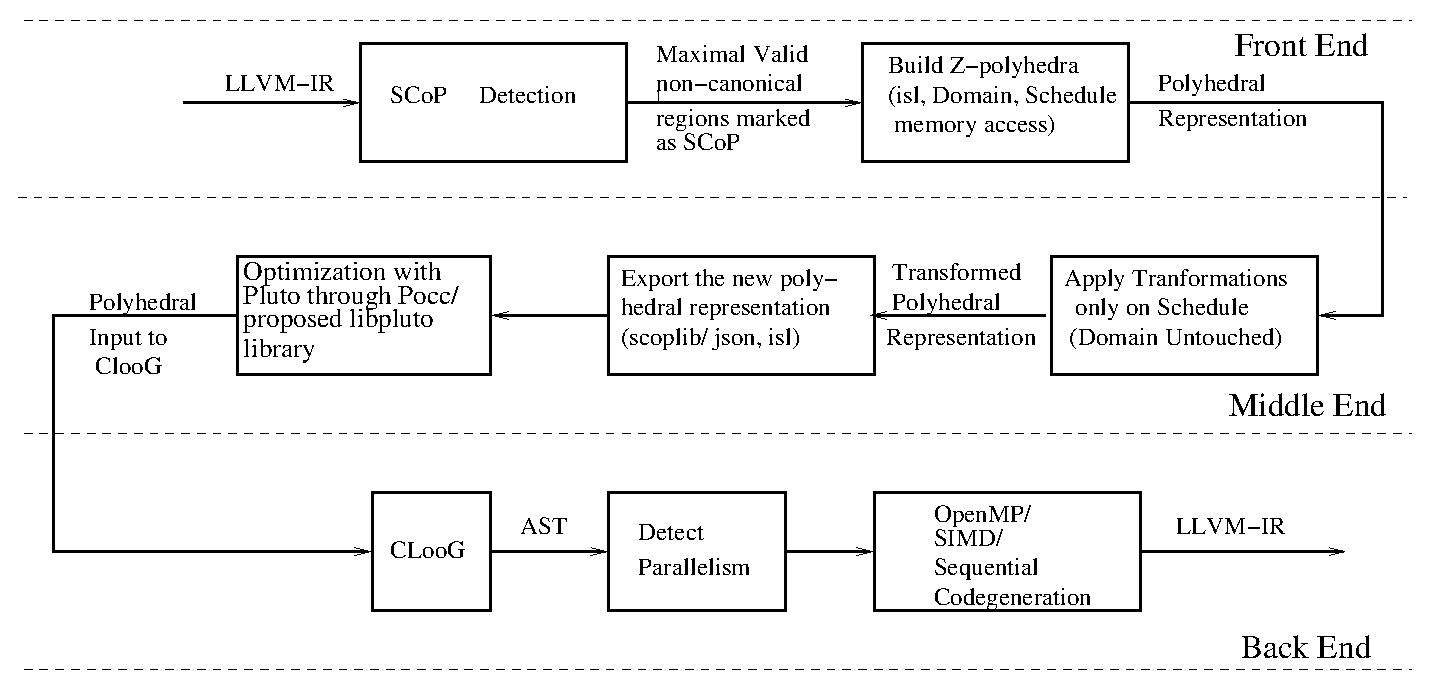
\includegraphics[width=1\textwidth]{images/detailedarch.eps}
  \caption{Detailed control flow in Polly}
  \label{detailed}
\end{center}
\end{figure}
Refer to the detailed control flow in Polly in Figure ~\ref{detailed}. Each of the module in Polly is
implemented as a LLMV pass\footnote{\url{http://llvm.org/docs/WritingAnLLVMPass.html}}. We have to generate the OpenMP code in the code 
generation pass of Polly(CodeGeneration.cpp). LLVM does the magic of running this code generation
pass for each of the detected SCoP. The runOnScop function initiates this. This function gather
the required information by running all passes(ScalarEvolution, LoopInfo, CloogInfo, SCopDetection, etc.).
The current pass can refer to the output of those passes as and when required. 

While generating the code for a loop we check whether this loop is parallel or not.  If it is
parallel instead of generating the normal sequential code,  loop is embedded in
libgomp library calls. The approach for detecting parallelism is explained in the next section.

\section{Detecting parallelism in Polly}

A common approach to detect
parallelism is to check before code generation, if a certain dimension of the
iteration space is carrying dependences. In case it does not, the dimension is
parallel.  This approach can only detect fully parallel dimensions. However,
during the generation of the AST, CLooG may split loops such that a
single dimension is enumerated by several loops.  This may happen
automatically, when CLooG optimizes the control flow.  With the classical
approach either all split loops are detected as parallel or no parallelism is
detected at all.

The approach taken in Polly detects parallelism after generating the generic
AST and calculates for each generated for-loop individually if it can be
executed in parallel. This is achieved by limiting the normal parallelism check
to the subset of the iteration space enumerated by the loop. To obtain this subset
we implemented an interface to directly retrieve it from CLooG. As a result,
we do not need to parse the AST to obtain it. With this enhanced parallelism
check parallel loops in a partial parallel dimension can be executed in
parallel, even though there remain some sequential loops. This increases the
amount of parallel loops that can be detected in unoptimized code and removes
the need for optimizers to place parallel and sequential loops in different
dimensions.

Polly automatically checks all generated loops and introduces OpenMP
parallelism for the outermost parallel loops. By default it assumes parallel
execution is beneficial. Optimizers that can derive that for some loops
sequential execution is faster may provide hints to prevent generation of
OpenMP code. Polly could incorporate such hints during code generation easily,
as they do not infect the correctness of the generated code.


\section{Generating OpenMP library calls}

Typically when a user want to run a particular section of the code in parallel he/she annotate the code with
OpenMP pragmas. The compiler will then convert this pragmas into the corresponding library calls. In Polly the
approach taken is to generate these calls automatically when a loop is detected as parallel.
Consider the for loop below to have a basic understanding about what is to be done.
{\footnotesize
\begin{lstlisting}
for (int i = 0; i <= N; i++)
  A[i] = 1 ;
\end{lstlisting}
}
This is detected as a parallel and given for OpenMP code generation. Here the following
sequence of GOMP library calls with proper arguments and return types(signature) has to be generated in
LLVM IR format. A general outline of the steps are given here and we enter into the implementation details.

\begin{itemize}
\item GOMP\_parallel\_loop\_runtime\_start
\item subfunction
\item GOMP\_parallel\_end
\end{itemize}

\begin{figure}
\begin{center}
  %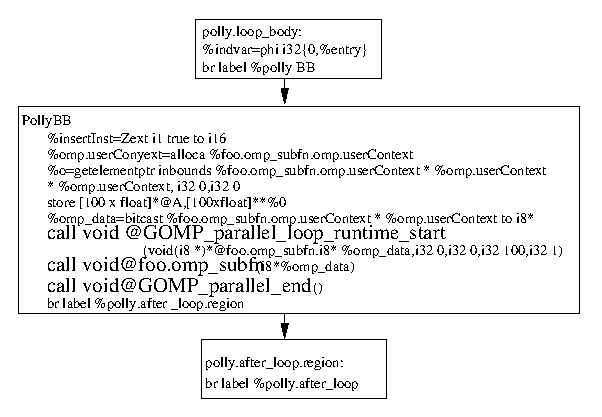
\includegraphics[width=1\textwidth]{images/ompcalls.eps}
  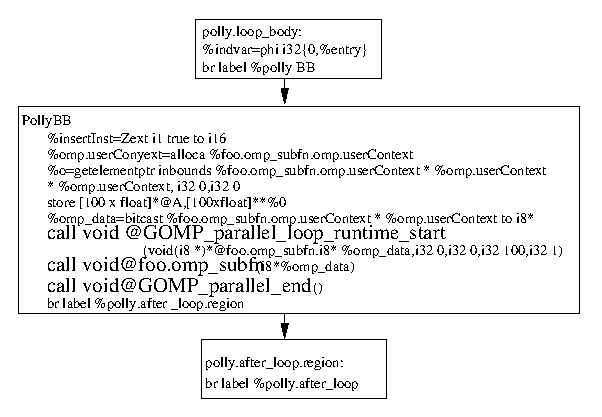
\includegraphics[width=14cm]{images/ompcalls.eps}
  \caption{CFG showing sequence of OpenMP library calls}
  \label{fig:openmp_cfg}
\end{center}
\end{figure}

The control flow graph corresponding to the previous example is shown in Figure ~\ref{fig:openmp_cfg}
The code for body of the for loop is generated inside the subfunction which has the following GOMP library
calls to achieve the necessary parallelism.

\begin{itemize}
\item GOMP\_loop\_runtime\_next
\item GOMP\_loop\_end\_nowait
\end{itemize}

The signature and descriptions of each of the above functions can be found in in libgomp manual\footnote{\url{http://gcc.gnu.org/onlinedocs/libgomp/}}.

The very first step is to create the prototype for each of the functions in LLVM-IR format\footnote{\url{http://llvm.org/docs/tutorial/LangImpl3.html\#funcs}}.
Code for generating prototype for "GOMP\_parallel\_end" is given below.
{\footnotesize
\begin{lstlisting}
Module *M = Builder.GetInsertBlock()->getParent()->getParent();
LLVMContext &Context = Builder.getContext();
if (!M->getFunction("GOMP_parallel_end")) {
  FunctionType *FT = FunctionType::get(Type::getVoidTy(Context), false);
  Function::Create(FT, Function::ExternalLinkage, "GOMP_parallel_end", M);
}
\end{lstlisting}
}
The first line gets the global module(M) where we store the information about the function to be created.
The 'Builder' function gives the current place to insert instructions. The 'FunctionType::get' method
puts the types of arguments and return type and 'Function::Create' create and insert the prototype
into the code. In a similar manner all the prototypes for other functions are created.

The next step is to insert calls to the library calls. These calls replaces the sequential code for
the original loop and the body of the loop is embedded in the OpenMP subfunction which is
going to be exectuted as an OpenMP thread. Here is the code to create call to "GOMP\_parallel\_end":
{\footnotesize
\begin{lstlisting}
Function *FN = M->getFunction("GOMP_parallel_end");
Builder.CreateCall(FN);
\end{lstlisting}
}

The next step which is more intersting is to create the body of the subfunction which involves the difficult process of
linking the basic blocks in proper manner. Here is the code to generate an empty body for the subfunction:
{\footnotesize
\begin{lstlisting}
LLVMContext &Context = FN->getContext();
// Create a new basic block to start insertion into.
BasicBlock *BB = BasicBlock::Create(Context, "entry", FN);
// Store the previous basic block.
BasicBlock *PrevBB = Builder->GetInsertBlock();
// Add the return instruction.
Builder->SetInsertPoint(BB);
Builder->CreateRetVoid();
// Restore the builder back to previous basic block.
Builder->SetInsertPoint(PrevBB);
\end{lstlisting}
}
This is just a basic code to create basic block 'BB' with label 'entry' The 'SetInsertPoint' function
can be used to insert code in a particular basic block. The complete control flow graph for the
subfunction body of a typical for loop will look like Figure ~\ref{fig:subfunction_cfg}. In the basic
block laballed 'omp.checkNext' we call "GOMP\_loop\_runtime\_next" which finds the upper and 
lower bound of each OpenMP thread. In the basic block with label 'polly.loop\_body' we
generate the sequential code for the loop.

\begin{figure}
\begin{center}
  \includegraphics[width=0.55\textwidth]{images/cfg2.ps}
%\includegraphics[width=14cm]{images/cfg2.ps}
  \caption{CFG showing basic blocks in the subfunction body}
  \label{fig:subfunction_cfg}
\end{center}
\end{figure}

\section{Support for inner loops}

So far OpenMP code created apply only for outermost loops, which is detected as SCoP. Next step is to do it for
inner loops. Due to dependency issues the outer loop is not detected as SCoP, but innerloop can be safely
parallelized as in the following example.
{\footnotesize
\begin{lstlisting}
for (int i = 0; i < M; i++)
  for (int j = 0; j < N; j++)
    A[j] += M;
\end{lstlisting}
}
Those loops need the values of the surrounding induction variables and parameters in the OpenMP subfunction. We need
to pass the values of the outer induction variables in a structure to the subfunction. All the required variables
were already available in a data structure used by Polly. We just needed to copy those into the body of the subfunction
so that it can refer those whenever needed.

\section{Dealing with memory references}
{\footnotesize
\begin{lstlisting}
#define N 10
void foo() {
  float A[N];
  for (int i=0; i < N; i++)
    A[i] = 10;
  return;
}
\end{lstlisting}
}
Consider the above code segment. The 'for' loop will be detected as parallel by Polly and will be embedded in the
body of the OpenMP subfunction. But it accesses a non-global array 'A' and so accessing the same will not be possible inside
the subfunction. The approach for solving this issue is explained below.

\subsection{Adding memory references}

The base addresses of all memory references made by a statement is available in each statement instance. Prior to creating the body
of the subfunction we add all these base addresses are added into the same data structure where we stored the induction variables and parameters.
And then it is added to the subfunction structure.

\subsection{Extracting memory references}

Inside the body of the subfunction the base addresses are extracted from the subfunction structure and a new LLVM load instruction is created for each. The
new base addresses mapped to the old addresses so that any future references are made on the new addresses.

\section{OpenMP testcases}

Polly follows the LLVM testing infrastrcutre\footnote{\url{http://llvm.org/docs/TestingGuide.html}} to add regression testcases. Testcases for OpenMP are added into
'test/Codegen/OpenMP' directory under Polly source tree. The tests can be carried out by just issuing the command 'make polly-test'
from the 'cmake' build directory.
